%
%   This program is free software: you can redistribute it and/or modify
%   it under the terms of the GNU General Public License as published by
%   the Free Software Foundation, either version 3 of the License, or
%   (at your option) any later version.
%
%   This program is distributed in the hope that it will be useful,
%   but WITHOUT ANY WARRANTY; without even the implied warranty of
%   MERCHANTABILITY or FITNESS FOR A PARTICULAR PURPOSE.  See the
%   GNU General Public License for more details.
%
%   You should have received a copy of the GNU General Public License
%   along with this program.  If not, see <http://www.gnu.org/licenses/>.
%

% Version: $Revision: $

%%%%%%%%%%%%%%%%
% Introduction %
%%%%%%%%%%%%%%%%

\section{Introduction}

From Weka 3.8.0 a new user interface called the Workbench is
available. The Workbench provides an all-in-one application that
subsumes all the major WEKA GUIs described in earlier sections. The
Workbench presents a set of ``perspectives'', where a perspective
might contain an entire application or individual panels/tabs from an
application. For example, the Explorer's main panels and plugin panels
all appear as separate perspectives in the Workbench, so at first
glance it appears very similar to the Explorer. However, other
perspectives can contain entire applications --- for example, the
Knowledge Flow or Experimenter.

\begin{center}
  \includegraphics[width=10cm]{images/workbench/workbench.eps}
\end{center}

Because the Workbench is made up of other applications, there is not
much further to describe here with respect to its functionality. One
exception is that the Workbench exposes a number of general and
perspective-specific settings and preferences that the user can
modify. Settings are accessible by either the gear shaped icon in the
upper left-hand side of the GUI, or from the ``Program'' menu.

\begin{center}
  \includegraphics[width=10cm]{images/workbench/settings.eps}
\end{center}

From the settings the user can choose which perspectives should appear, and
modify general settings, such as the look-and-feel to use. Some settings
will come into affect immediately; while others, such as the look-and-feel,
will require that WEKA is restarted after making the change.

Beyond the \textit{Perspectives} and \textit{General} tabs in the settings
dialog each perspective will have its own tab for settings (as long as
a given perspective has user-configurable settings).

\begin{center}
  \includegraphics[width=10cm]{images/workbench/settings2.eps}
\end{center}

\begin{center}
  \includegraphics[width=10cm]{images/workbench/settings3.eps}
\end{center}
